\documentclass[14pt]{beamer}

\title[SlideSpeak]{The Infanzia Series}
\subtitle{Interactive Fun Learning Apps for kids}
\author[Team 16]{Rishika J; Sonal K; Akansha MP}
\date{July 2020}

\usetheme{metropolis}
\usecolortheme{wolverine}
\usepackage{graphicx}
\usepackage{xcolor}

\begin{document}


\begin{frame}
    \titlepage
\end{frame}


\begin{frame}{Overview}
    \pause
    \begin{itemize}
    \item \textbf{Motive}: \\
            Interactive Enjoyable Applications
        \pause
    \item \textbf{Target Audience}: \\
            Pre-schoolers and Kindergartners
    \end{itemize}
\end{frame}

\begin{frame}{Techstack}
    \pause
    \begin{enumerate}
        \item Flutter
        \item Dart Language
        \item Firebase  
    \end{enumerate}
\end{frame}

\begin{frame}[standout]
    The Infanzia Series Apps: 
    \pause
    \alert{Word-it-Kid: English} \\
    \pause
    \alert{Count-it-Kid: Maths} \\
    \pause
    \alert{Know-it-Kid: EVS} 
\end{frame}

\begin{frame}{Word-it-kid :: Login Page}
    \begin{figure}[ht]
    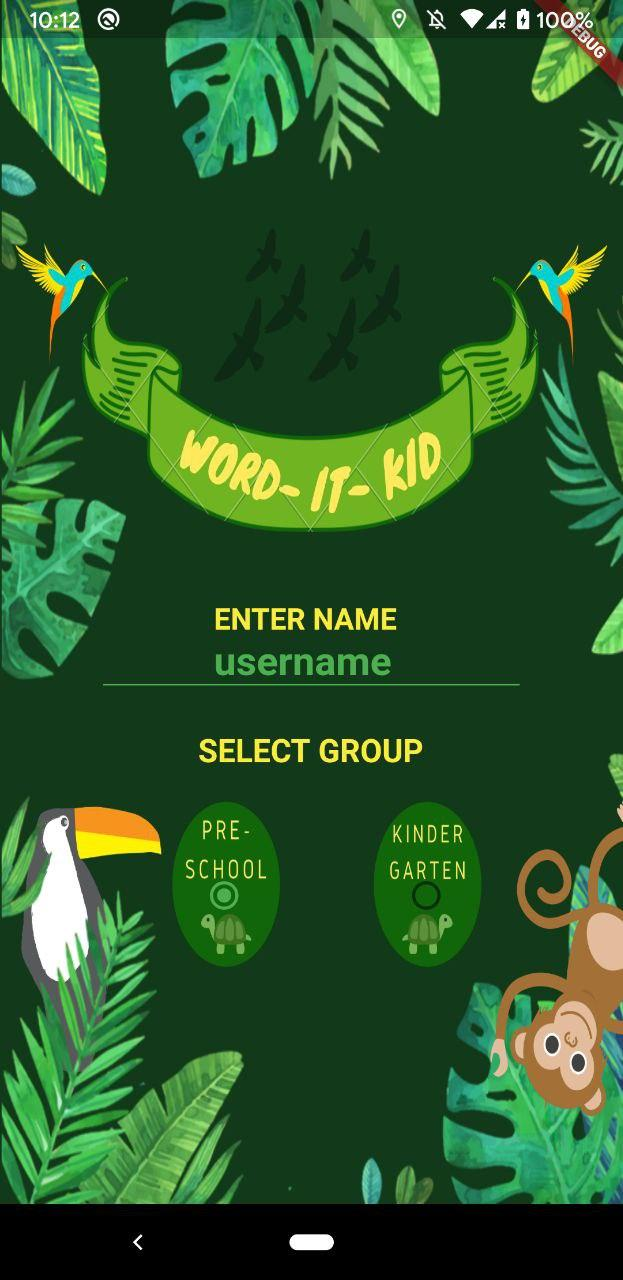
\includegraphics[height=3in]{LoginPage.JPG}
    \end{figure}
\end{frame}

\begin{frame}{Word-it-kid :: Main Page}
    \begin{columns}
    \begin{column}{0.4\textwidth}
        \begin{itemize}
            \item Learn with fun exercises \\
            \item Play games \\
            \item Sing along rhymes
        \end{itemize}
    \end{column}
    \begin{column}{0.6\textwidth}
        \begin{figure}[ht]
        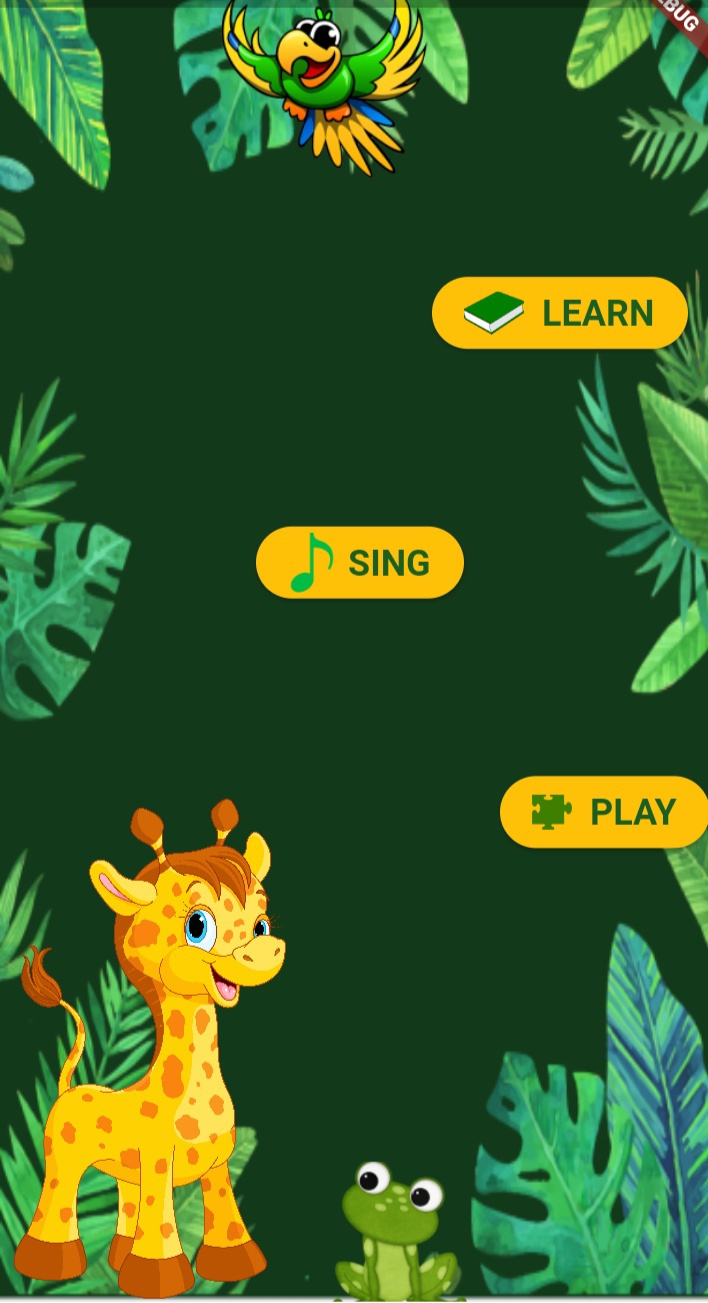
\includegraphics[height=3in]{RedirectionPage.jpeg}
        \end{figure}
    \end{column}
    \end{columns}
\end{frame}

\begin{frame}{Status}
\end{frame}


\end{document}
